\renewcommand{\chaptername}{Requerimientos para estación terrena}
\chapter{Posicionador para antena }
%encabezado 
\markright{posicionador para antena}
%----------Abstract del capitulo ----------------------------%
\begin{center}
\begin{tcolorbox}[colback=gray!5!white, %Color del fondo
colframe=gray!75!black,
title= \center{\Large{Resumen}} ]

Se definen los requerimientos del sistema y las necesidades del radiobservatorio. Además, se muestra una planificación del trabajo a lo largo de este texto. 
\end{tcolorbox}
\end{center}    
%-------------Fin de abstract de capitulo ----------------------%
\section{Introducción}  %\label{cap1:introduccion}
En el marco de la cátedra Proyecto Final de la carrera de ingeniería electrónica, de la fac. de ingeniería, perteneciente a la Universidad Nacional De La Plata, se diseña un sistema electrónico para el  posicionamiento de una antena, cuyo lugar de realización es el Instituto Argentino de Radioastronomía(IAR), en la modalidad con director. Este instituto, se dedica a la radioastronomía, que es la observación del cielo mediante ondas de radio. Dicha institución, quiere realizar la bajada de datos satelitales, medir la potencia total, vender el servicio a terceros, velar por el cumplimiento de normas internacionales, etc. Para tal fin se emplea un receptor de comunicaciones adosado a una antena parabólica en desuso para obtener estos datos.

La antena, posee un radio de 2 metros aproximadamente, la misma tiene un sistema mecánico, que mueve la antena mediante dos motores, en dos ejes independientes entre sí. Se describen los trabajos realizados para recuperar los motores de la antena, desarrollo del sistema electrónico y software de posicionamiento y bajada de datos satelitales. Por lo expuesto en el párrafo anterior, el sistema, para realizar la bajada de datos satelitales, debe realizar el seguimiento de satélites que se encuentren dentro de los ángulos de visibilidad de la antena.

\section{Instituto Argentino de Radioastronomía} 

El Instituto Argentino de Radioastronomía(IAR),posee dos antenas parabólicas(ver figura \ref{fig_antena}, donde se aprecia la antena de fondo), de 30 mts de diámetro aproximadamente, las cuales son utilizadas para observaciones astronómicas. La emisión de potencia de los satélites, puede interferir en las observaciones astronómicas, y podrían realizarse filtros adaptativos, para estos receptores. Otra posible aplicación es la venta de estos datos a privados, verificar el cumplimiento de normas de potencia emitida (velando por el correcto uso del espacio radioeléctrico) por satélites, y un sin fin de aplicaciones. 

Para realizar esta medida de potencia, el IAR, requiere el seguimiento de los satélites que se encuentren dentro de la visibilidad que posea la antena, para poder medir esta potencia total y realizar un cálculo de la potencia emitida por los mismos. En la imagen \ref{fig_antena} se muestra la antena sobre la que se realiza el trabajo, y de fondo, una de las antenas principales de la institución.   

\begin{figure}[h]
	\centering 
	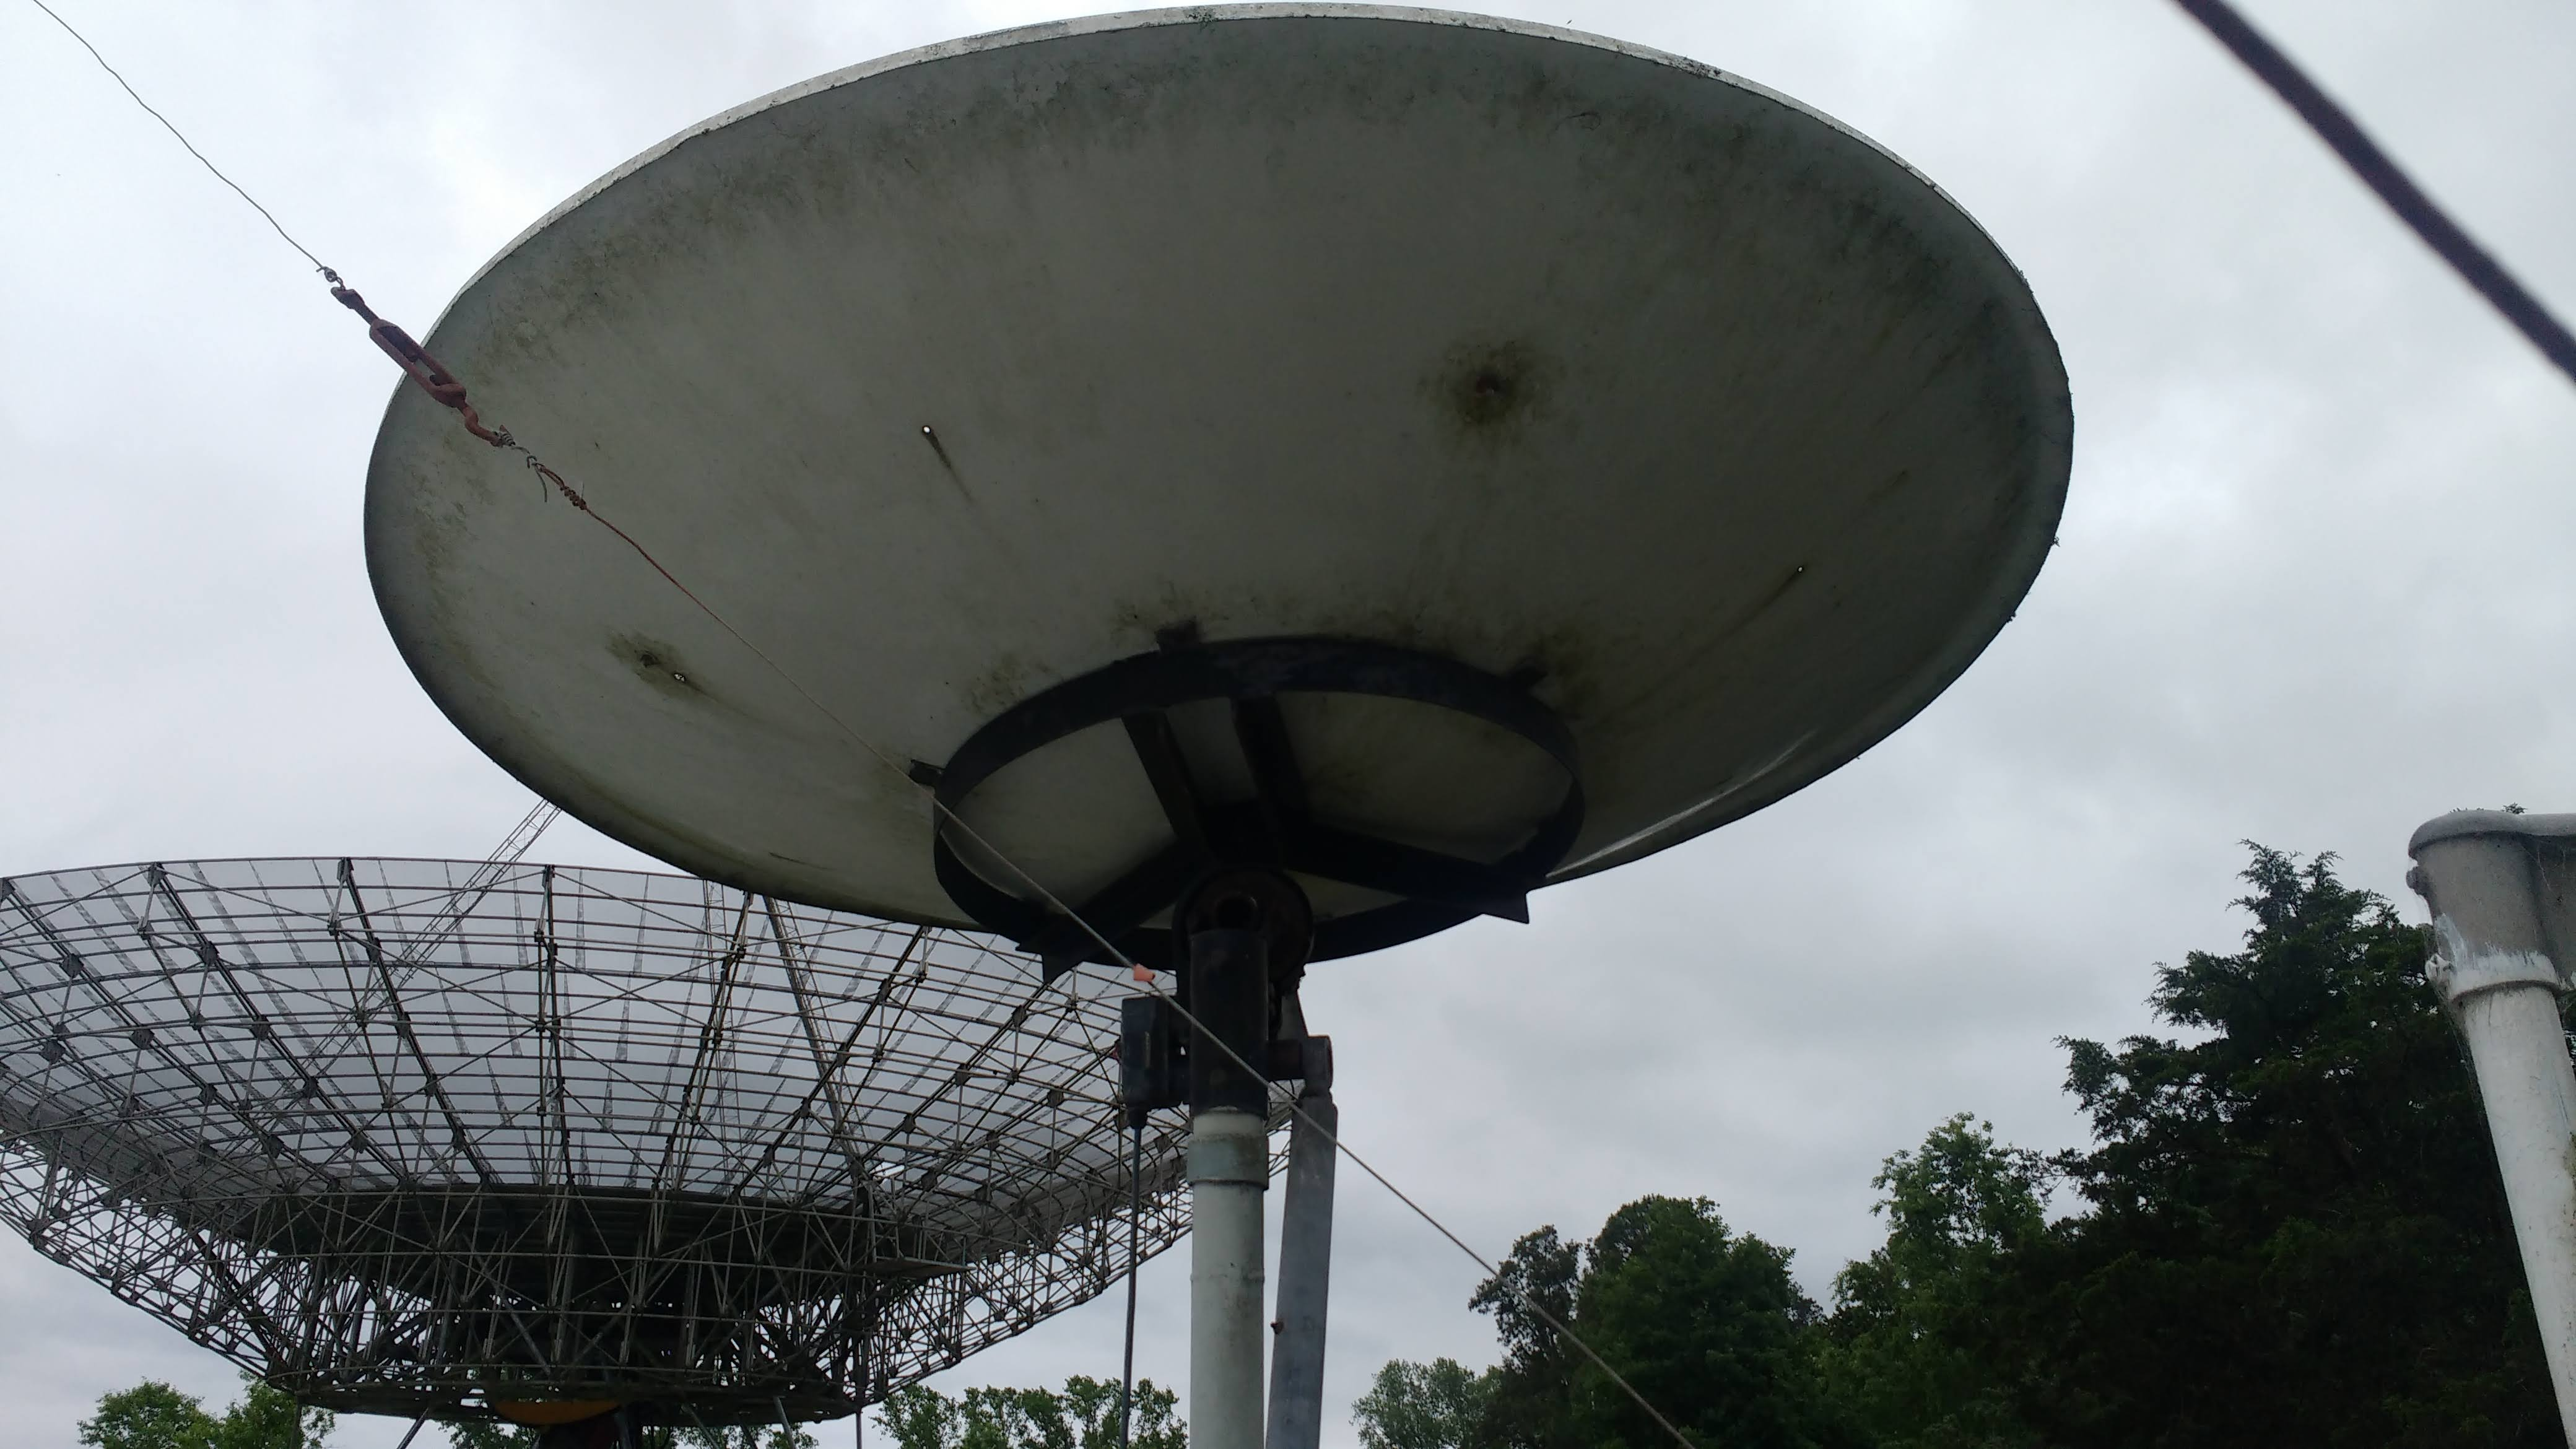
\includegraphics[width=0.5\textwidth]{parte_1/cap1/antena}
	\caption{antena ubicada en el iar, actualmente en desuso}
	\label{fig_antena}
\end{figure}

\section{Descripción de la Antena y posicionador }

La antena tiene el sistema mecánico que se observa en la figura \ref{fig_mec_ant}. 
% iamgen de la mecánica de la antena 
\begin{figure}[ht]
	%\centering 
	\begin{subfigure}{0.5\textwidth}
		\centering
		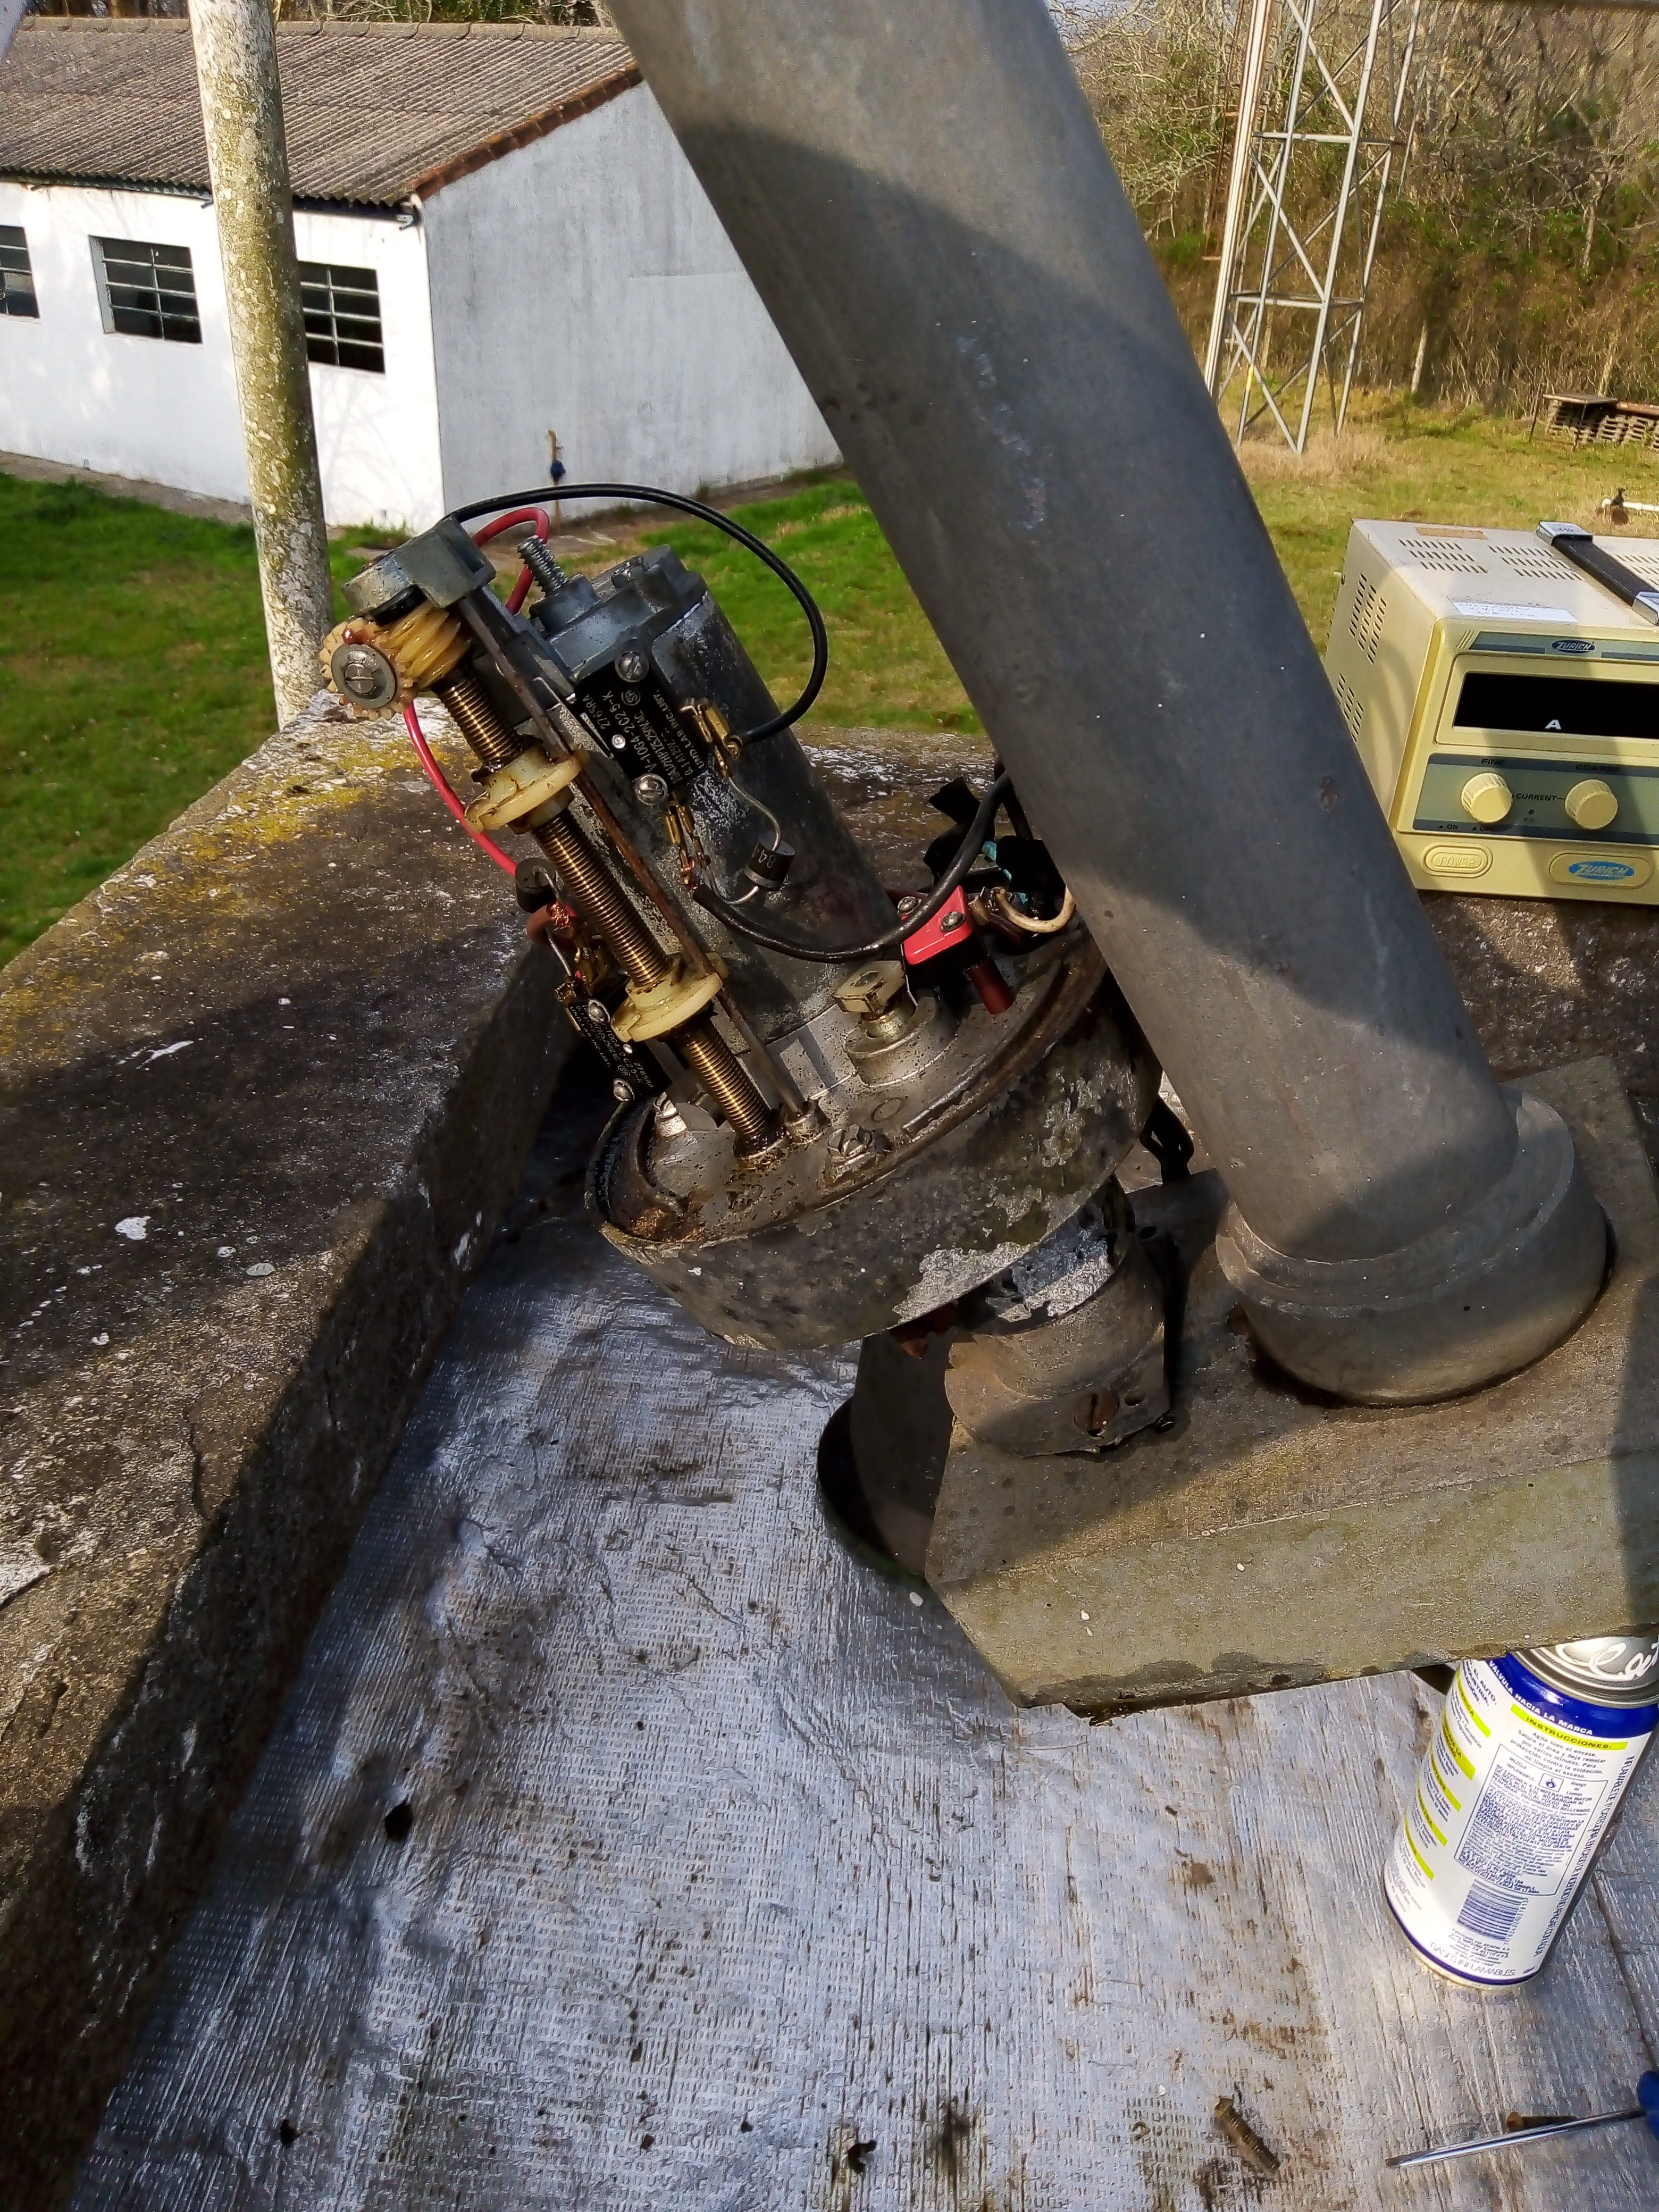
\includegraphics[width=0.5\textwidth]{parte_1/cap1/mot1}
		\caption{Motor del primer eje de la antena }
		\label{fig_mec_ant1}		
	\end{subfigure}
	\hfill 
	\begin{subfigure}{0.5\textwidth}
		\centering
		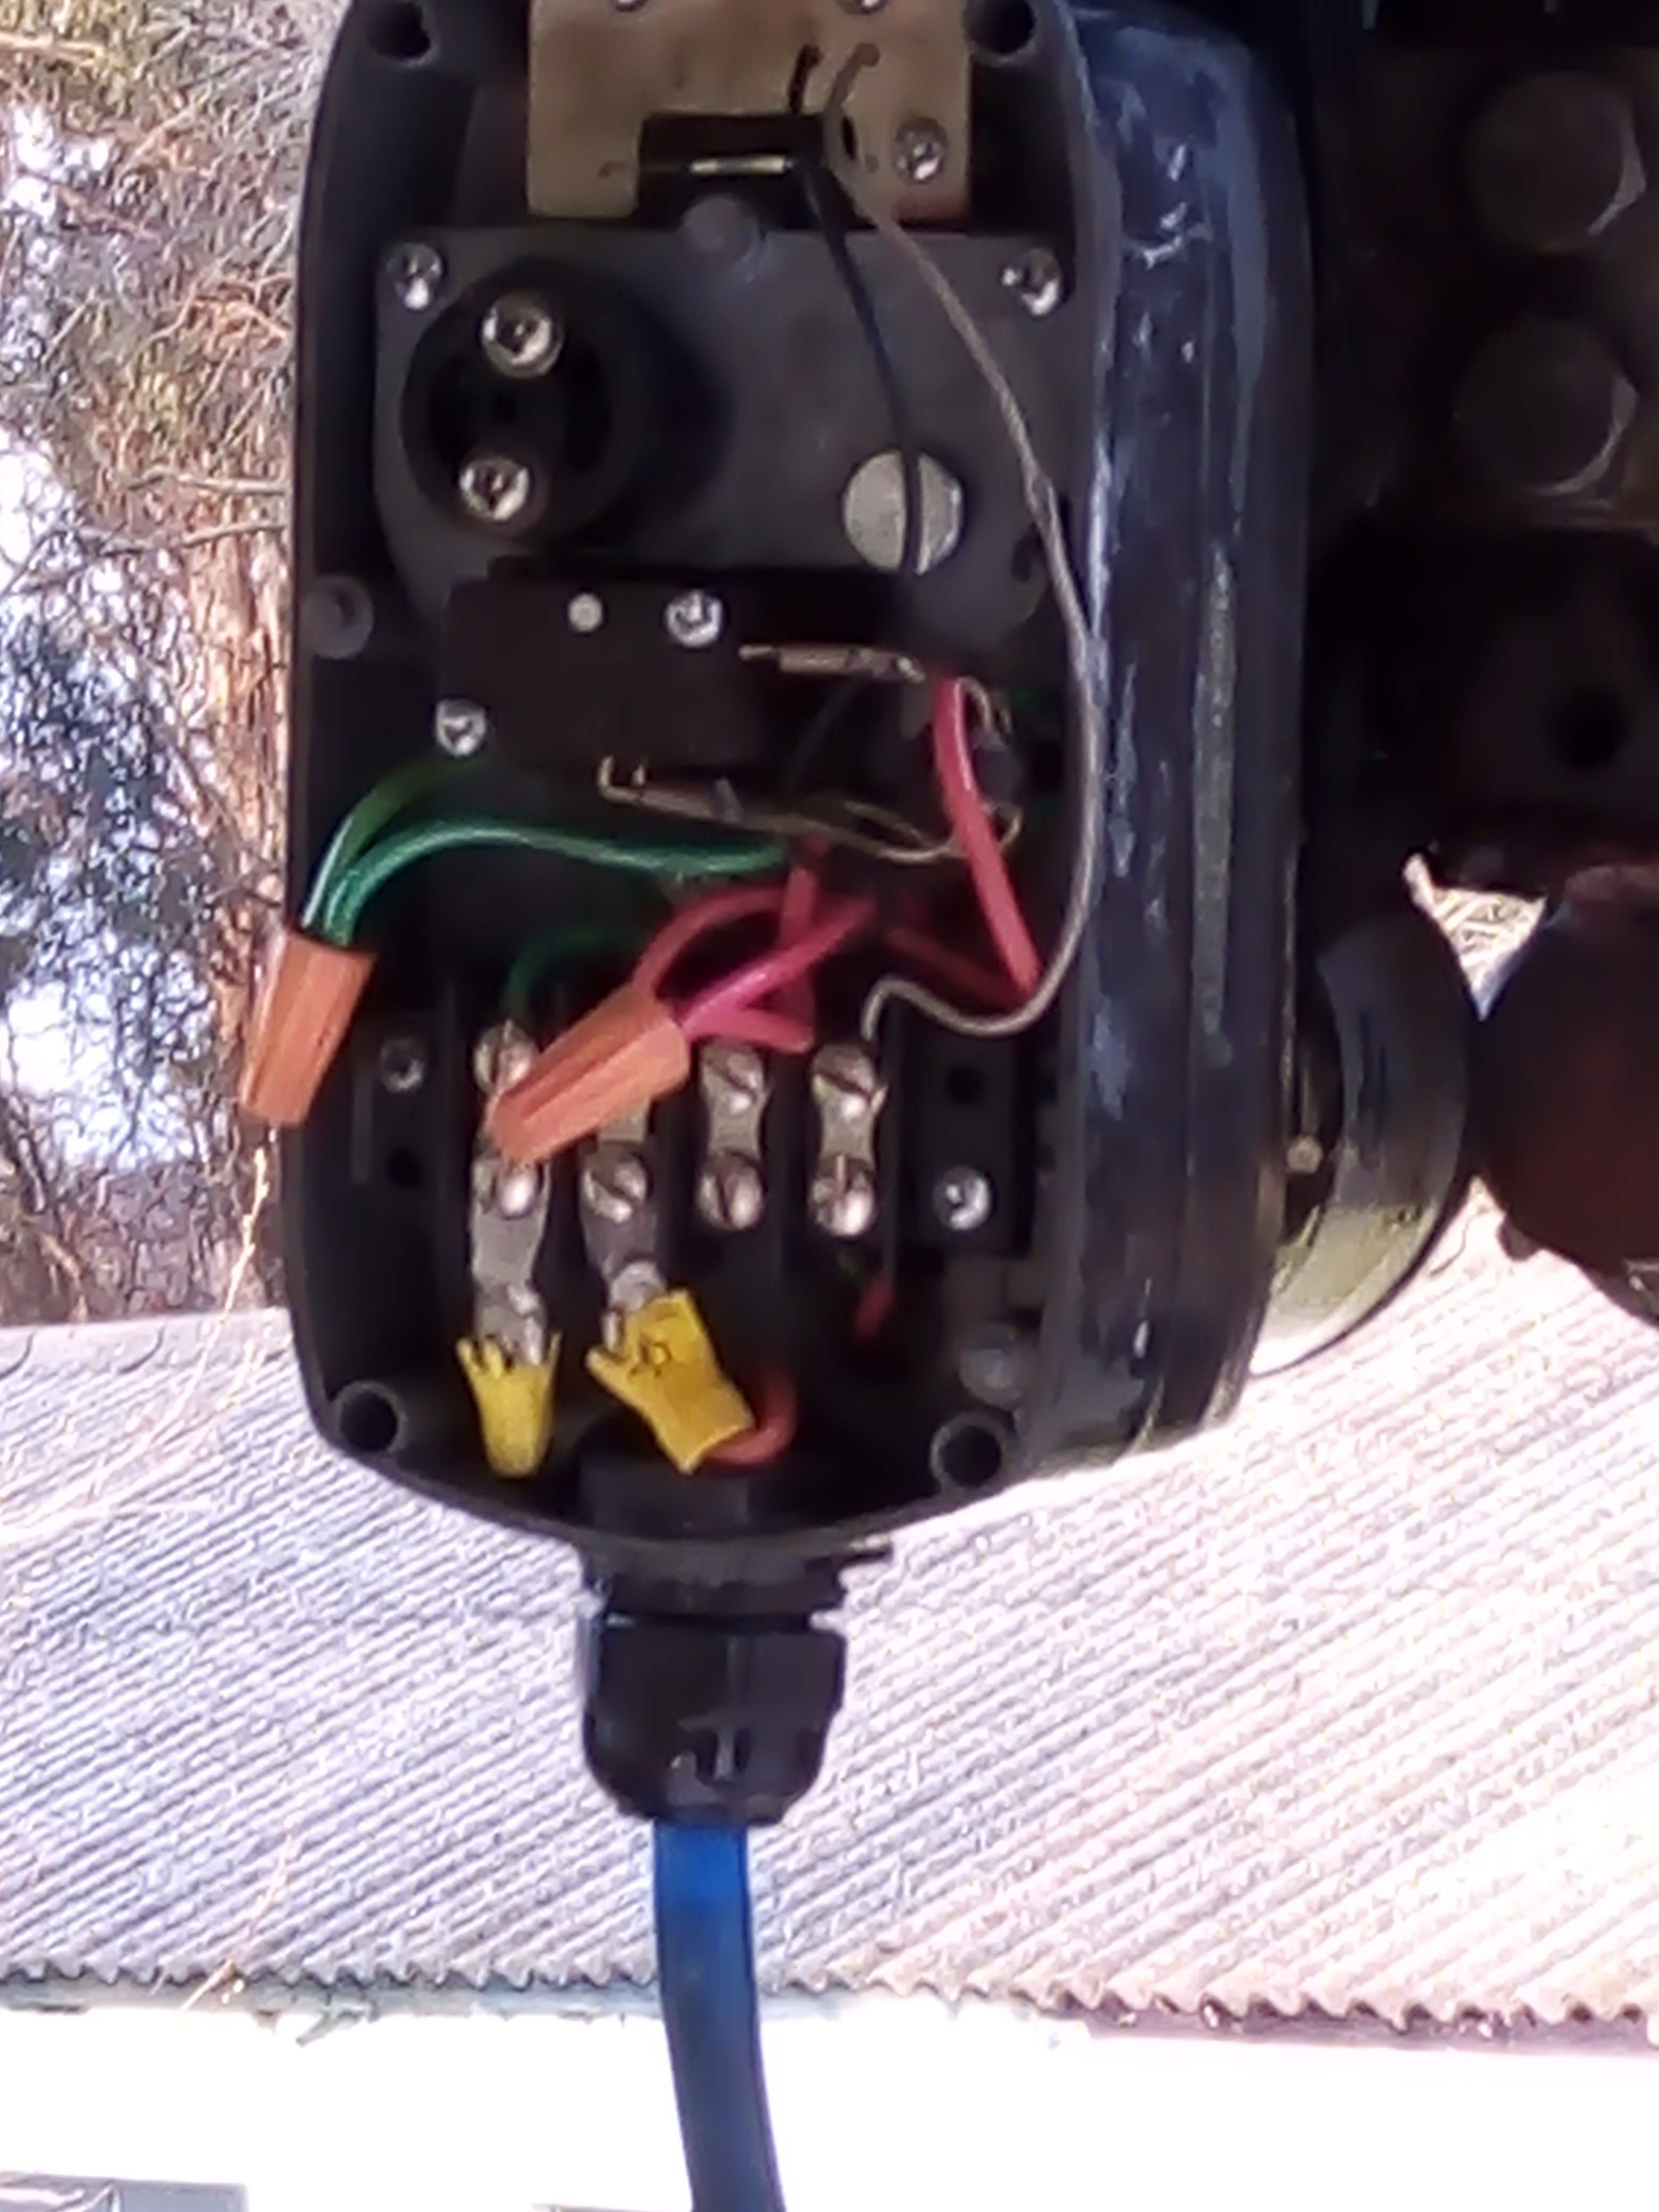
\includegraphics[width=0.5\textwidth]{parte_1/cap1/mot2}
		\caption{Motor del segundo eje de la antena }
		\label{fig_mec_ant2}
	\end{subfigure}
	
	\caption{Encoders asocioados a los motores de las antenas.}
	\label{fig_mec_ant}
\end{figure}


La antena cuenta con dos motores, uno por cada eje de movimiento, independientes entre sí: altura y azimut. Cada eje cuenta, además, con la medición de posición mediante un potenciómetro, con el que se realimenta al sistema de posicionamiento. 

En el presente trabajo, se va a desarrollar un sistema que sea capaz de realizar el movimiento de la antena, aprovechando el sistema de motores existente sobre la misma. El sistema, que realiza el movimiento de la antena, se conoce como ``posicionador''. Este sistema, recibe una posición, en dos coordenadas, y tiene que mover la antena hacia las coordenadas recibidas. Estas coordenadas que recibe, son las posiciones de los satélites, los cuales se van moviendo, por ende, mientras el satélite este por encima de la antena, o su ``horizonte visible'', debe realizar el seguimiento de la misma, actuando sobre los motores, y acomodando la antena, a donde este el satélite en cuestión.

En la actualidad, existen diversos programas para realizar el seguimiento de satélites en tiempo real, estos consultan bases de datos existentes en Internet, y realizan el cálculo en base a modelos matemáticos. En este documento, se hará uso de alguno de estos programas, para poder actualizar la posición a cada instante y mover los motores hacia donde corresponda. Además, este dispositivo, debe ser controlador desde una PC que esté ubicada dentro de la institución. 

\section{Metodología de trabajo}

El trabajo, se divide  en cuatro etapas, denominadas ``fase 1, fase 2, fase 3 y fase 4'' respectivamente. En la primera fase, se va a definir los requerimientos del sistema(capítulo actual), luego se va a proponer una solución a para cumplir estos requerimientos(cap. 2 ), y luego se van a seleccionar algunas piezas electrónicas para la construcción de la solución(cap 3.). 

En la segunda fase, se va a desarrollar el software que debe realizar el sistema de control, tanto para el usuario, como para la computadora que controla la antena. El orden del trabajo, es primero decidir qué softwares se usarán sobre la/s computadoras de la institución, y luego programar el microcontrolador o PC que realiza el control sobre la antena.

En la tercera fase, se va a realizar una investigación sobre los sistemas de coordenadas y como se realizan las transformaciones de estas entre sí.

En la cuarta fase, se va a desarrollar el sistema de posicionamiento de los motores, luego se desarrolla la interfaz para conectarse a la computadora que realiza el control del sistema. Luego, una vez desarrollado estas interfaces, se prueba el sistema realizando algún seguimiento, sea a satélites, o a estrellas, o realizando algún apuntamiento de tipo manual. Estas fases, y capítulos a lo largo del texto, se resumen en la siguiente tabla:    


\renewcommand{\arraystretch}{1.5}

% tabla 
\begin{table}[ht]
	\centering
	\begin{tabular}{|c|c|p{8cm}|}
		\hline
		Fase & Capítulos & Descripción de la fase \\
		\hline 
		\multirow{3}{2cm}{Fase 1} & capítulo 1 & {Definición del proyecto} \\ \cline{2-3}
		& capítulo 2& Definición de los componentes que requiere el proyecto\\ \cline{2-3}
		& capítulo 3& Selección de los componentes de hardware, en base a requerimientos\\ \hline 
%---------------- segunda fase 		
		\multirow{3}{2cm}{Fase 2} & capítulo 4 & Estudio de redes de computadoras \\ \cline{2-3}
		& capítulo 5& Software sobre la PC para el usuario final.\\ \cline{2-3}
		& capítulo 6& Programación del microcontrolador, y conexión con Gpredict y Stellarium\\ \hline 
		

%---------------- tercera fase 		
	   \multirow{2}{2cm}{Fase 3} & capítulo 7 & Sistemas de coordenadas esféricos\\ \cline{2-3}
	   & capítulo 8& Implementación de los sistemas de coordenadas esféricos dentro del microcontrolador.\\ \cline{2-3} \hline 
	   
%---------------- cuarta fase 		
	\multirow{2}{2cm}{Fase 4} & capítulo 9 & Desarrollo de un controlador para los motores de la antena\\ \cline{2-3}
	& capítulo 10& Resultados y conclusiones del trabajo - Futuras versiones\\ \cline{2-3} \hline 
	\end{tabular}
	\caption{Resumen del trabajo en cada fase del proyecto}
\end{table}


\section{ Requerimientos del sistema} \label{req_sist}

De lo expuesto en las secciones anteriores, podemos obtener los requerimientos para este proyecto. Los requerimientos para este proyecto se dividen en dos tipos:  
\begin{enumerate}
	\item Requerimientos funcionales: se definen aquellas cosas relacionadas al comportamiento del dispositivo a diseñar  
	\item Requerimientos de sistema: se refiere a como llevar a cabo la solución en sí.  
\end{enumerate} 
%\renewcommand{\multirowsetup}{\centering}
La siguiente tabla, contiene una lista de ambos requerimientos:  
\renewcommand{\arraystretch}{1.5}

\begin{table}[H]
\begin{tabular}{|c|c| p{10cm} | }
% REQUISITOS FUNCIONALES 
	 \hline 	 
	 \multirow{11}{*}[-0.5cm]{\rotatebox[origin=c]{90}{\centering Requerimientos}} 
	 &\multirow{5}{*}[-0.25cm]{\centering Requisitos funcionales} & Medir posición de la antena. \\ \cline{3-3}
	 & & Recibir coordenadas desde una PC dentro del IAR. \\ \cline{3-3}
	 & & Tener control sobre la posición de la antena.\\  \cline{3-3}
	 & & Estacionar la antena en la posición del Cenit cuando no realice seguimientos sobre satélites. \\    \cline{3-3}
	 & & Seguimiento de satélites, naturales y artificiales, y estrellas. \\ \cline{3-3}
	 \cline{2-3}
% REQUISITOS DE SISTEMA 
	 &\multirow{6}{*}[-0.4cm]{\centering Requisitos De Sistema} & No puede utilizar ningún tipo de red inalámbrica. \\ 
	 \cline{3-3}	
	 & & Existencia de componentes en el mercado local. \\
	 \cline{3-3}
	 & & Escalable. \\ \cline{3-3}  
	 & & Independencia entre los componentes del sistema. \\ \cline{3-3}
	 & & Calibración automática del sentido de movimiento y posiciones angulares. \\ \cline{3-3}
	 & & Bajo costo. \\
	 \hline 
\end{tabular}
\caption{Requerimientos del sistema }
\label{tab:requerimientos}
\end{table}








% imagen de la antena La tabla anterior, nos brinda los requerimientos, sobre los cuales se va a desarrollar el sistema de posicionamiento para la antena en cuestion. Los requerimientos, están de acuerdo, a la necesidad de la institución. 





 

 
%------------Final capitulo 1 ------------------------------%  



